\FloatBarrier
\subsection{Kurvenauswertung}

Wie in der Vorbereitung geschrieben werden die aufgenommenen Kurven nun ausgewertet. Insgesamt wurden sieben aufgenommen, drei für die Längsspannung und vier für die Querspannung. Eine Datei für die Längsspannung wurde nicht gespeichert. Der Grund dafür ist uns nicht klar, die handschriftlichen Aufzeichnungen sind vollständig. \\
Die Längsspannung wurde jeweils an den Stellen 2 und 6 abgegriffen, die Querspannung zwischen 3 und 4.

\subsubsection{Längsspannung}
Für die Längsspannung wurden die Kurven, die in Abb.2-4 zu sehen sind, aufgenommen. Zur Bestimmung der Maxima wurden Fits einer Gauß-Kurve in einem begrenzten Wertebereich gefittet. Die so bestimmten Werte sind in Abb.1 tabellarisch dargestellt.


\begin{figure}
\centering
\caption{Spannungswerte und Magnetfeldstärken an den Maxima.}
\vspace*{0.5cm}
\begin{tabular}{cccc}
\hline
Stromstärke in $\mu A$ & Temperatur in $K$ & B in $T$ & U in $V$ \\
\hline
\hline
20  & 4.4  & $1.831 \pm 0.004$ & 0.021 \\
	&		& $3.292 \pm 0.004$ & 0.048 \\
100 & 4.4  & $1.855 \pm 0.004$ & 0.094 \\
	&		& $3.455 \pm 0.003$ & 0.195 \\
100 & 2.95  & $2.369 \pm 0.007$ & 0.095 \\
	&		& $4.406 \pm 0.006$ & 0.202 \\
\hline
\end{tabular}
\end{figure}

%T_high I_low U_längs
%B1 = 1.83143 +- 0.00449283
%U1 = 0.02058
%B2 = 3.29231 +- 0.00382163
%U2 = 0.04827
\begin{figure}
\label{}
\centering
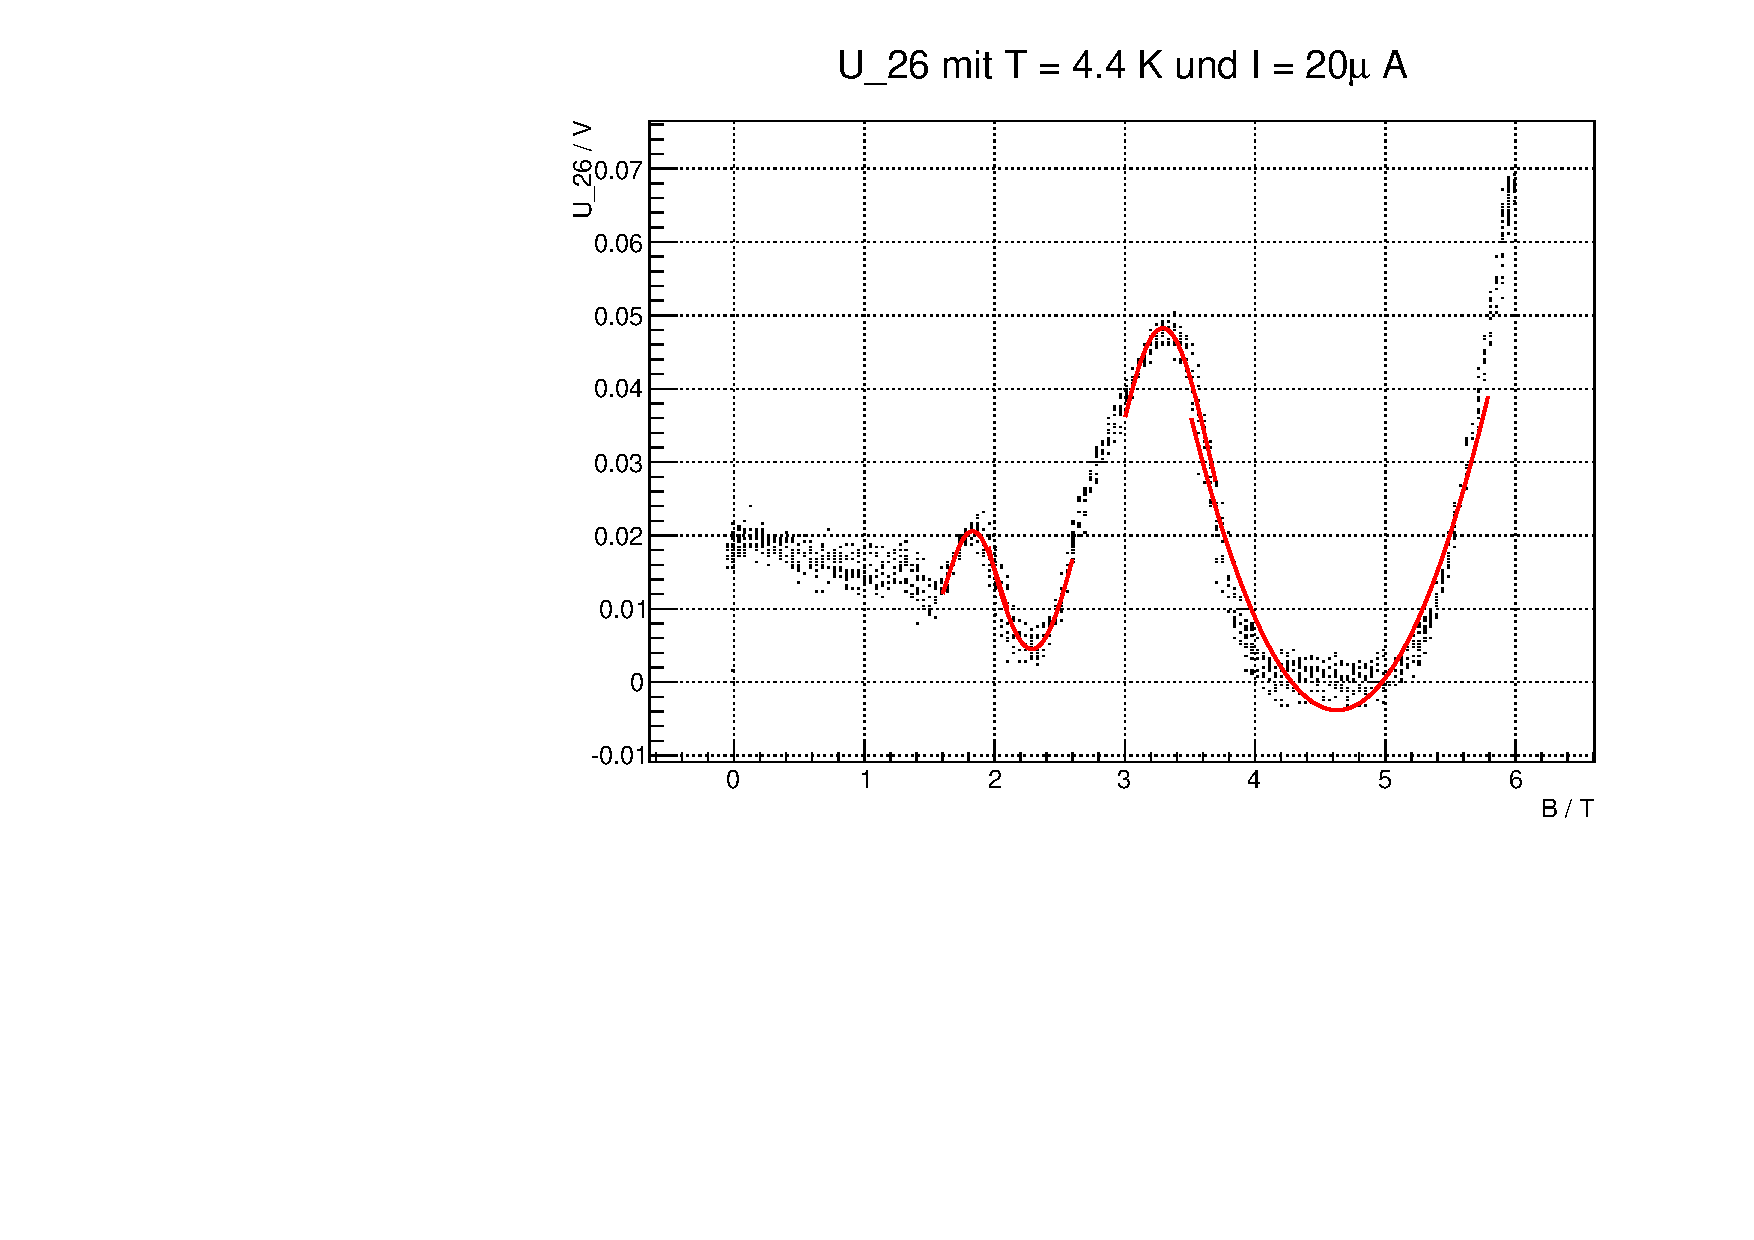
\includegraphics[scale = 0.5]{../plots/U_26_20muA_4400mK.pdf}
\caption{Längsspannung $\text{V}_x$ für I=20 $\mu$A und T=4.4 K}
\end{figure}

%T_high I_high U_längs
%B1 = 1.85495 +- 0.00420536
%U1 = 0.09374
%B2 = 3.45507 +- 0.00343915
%U2 = 0.19468
\begin{figure}
\label{}
\centering
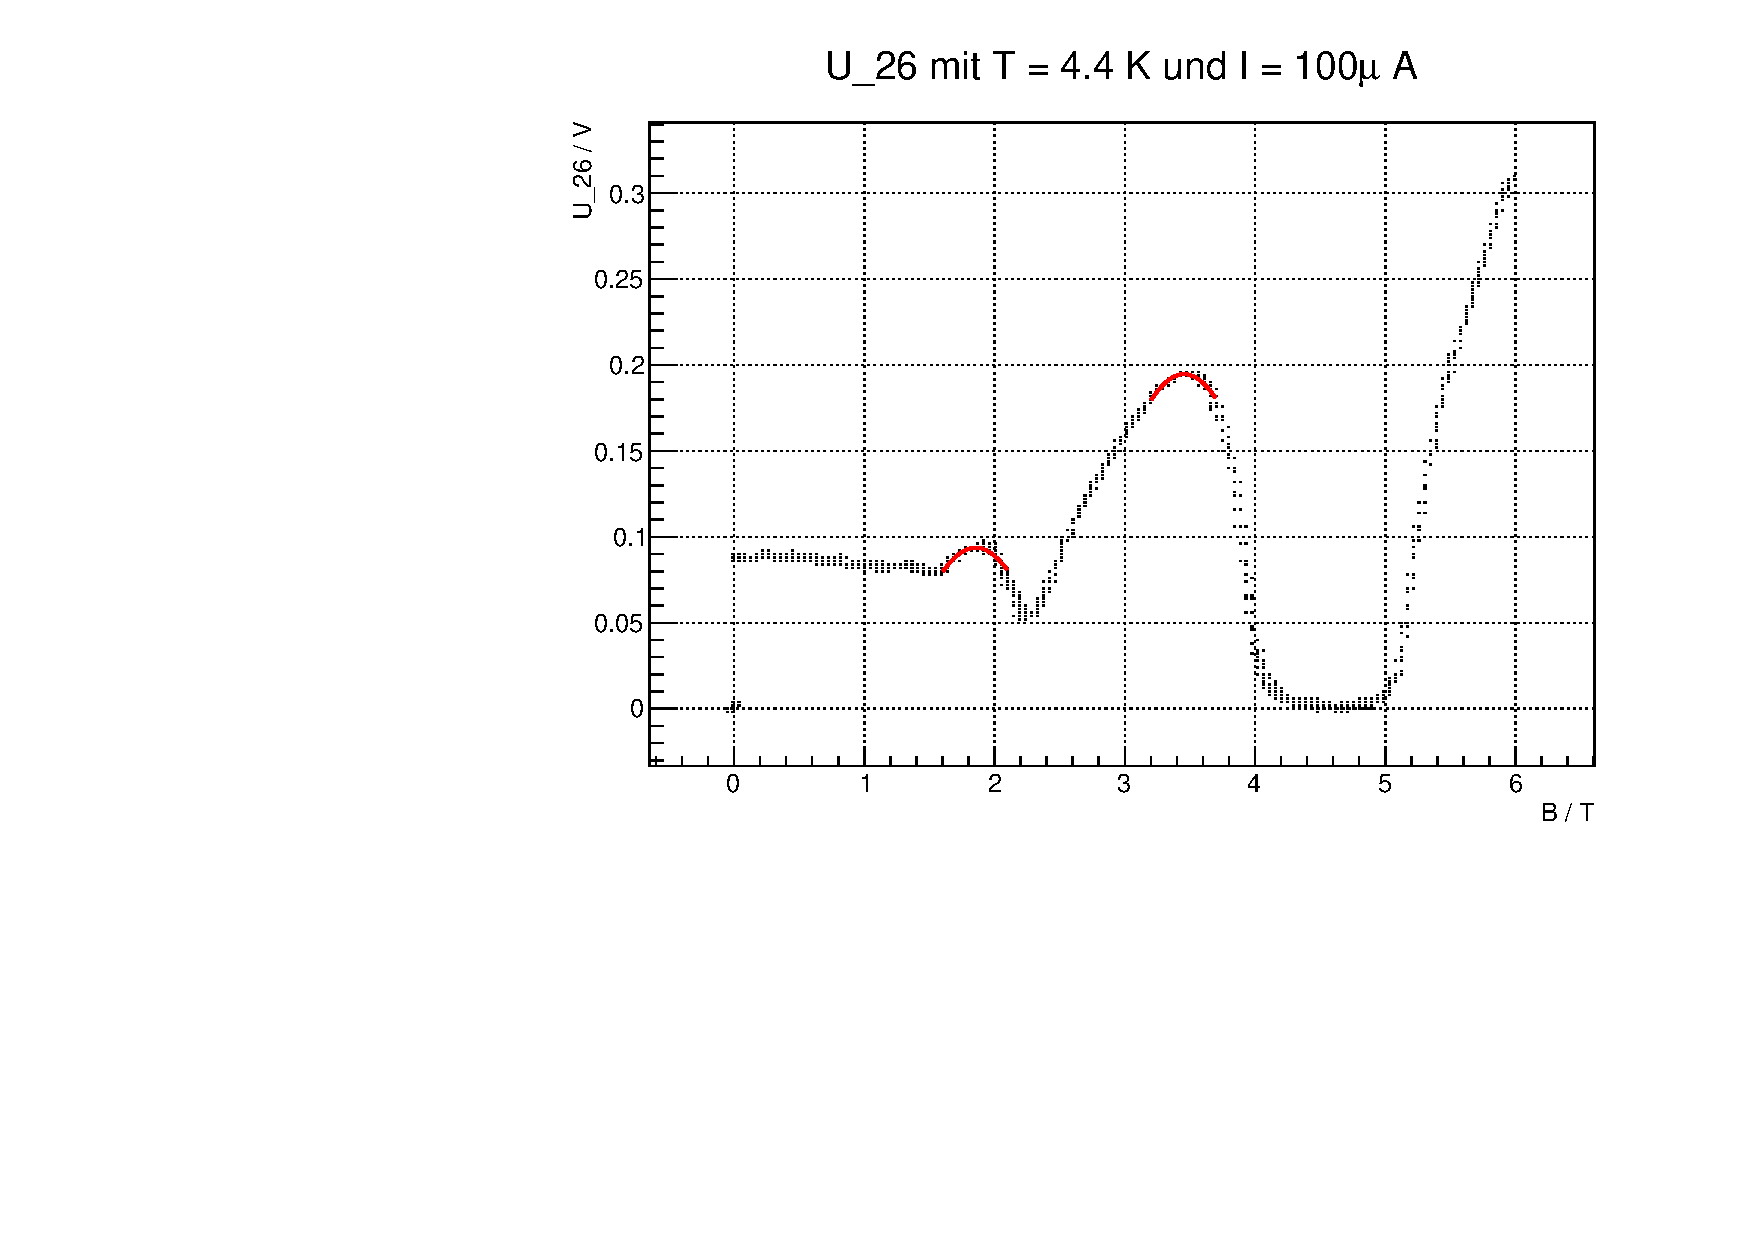
\includegraphics[scale = 0.5]{../plots/U_26_100muA_4400mK.pdf}
\caption{Längsspannung $\text{V}_x$ für I=100 $\mu$A und T=4.4 K}
\end{figure}

%missing
%%T_low I_low U_längs
%\begin{figure}
%\label{}
%\centering
%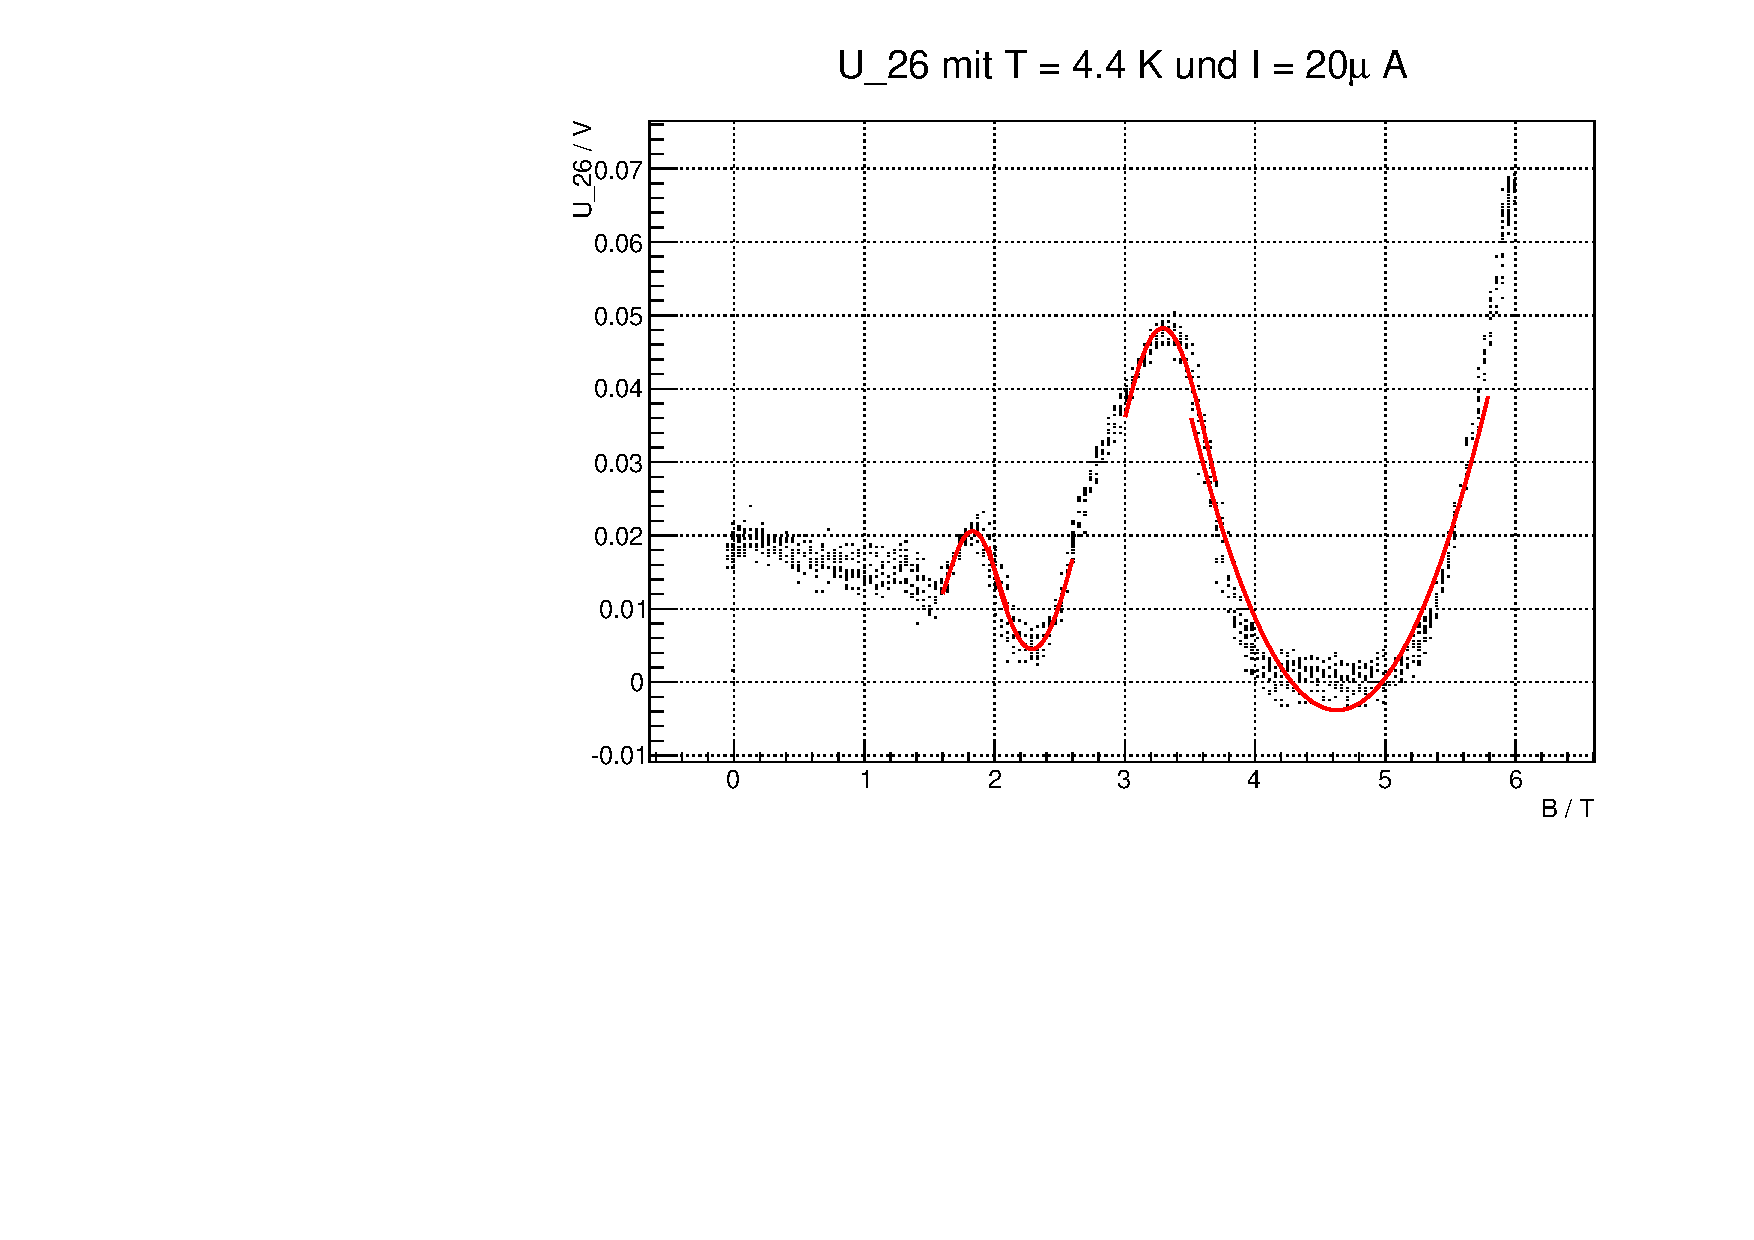
\includegraphics[scale = 0.5]{../plots/U_26_20muA_4400mK.pdf}
%\caption{}
%\end{figure}

%T_low I_high U_längs
%B1 = 2.36875 +- 0.00691555
%U1 = 0.095265
%B2 = 4.40606 +- 0.00615656
%U2 = 0.202313
\begin{figure}
\label{}
\centering
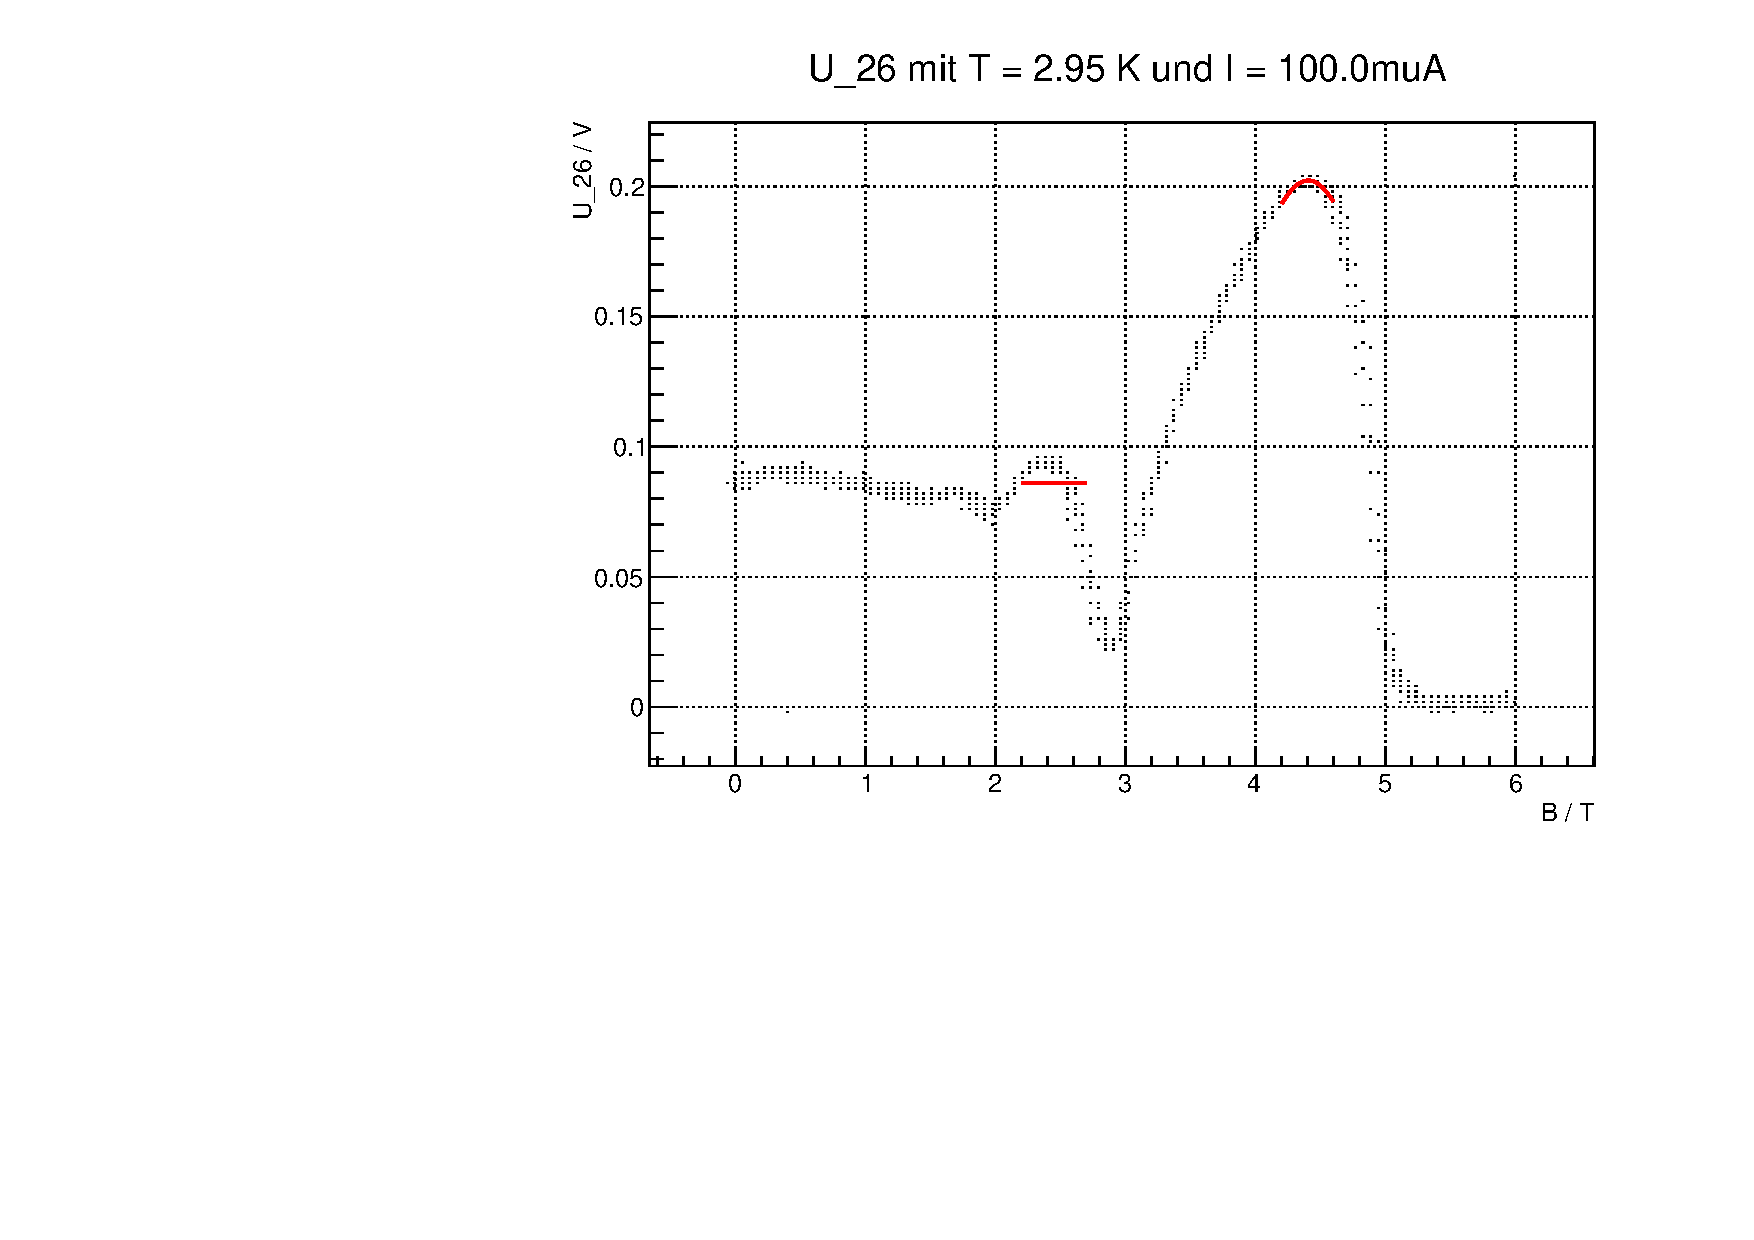
\includegraphics[scale = 0.5]{../plots/U_26_100muA_2950mK.pdf}
\caption{Längsspannung $\text{V}_x$ für I=100 $\mu$A und T=2.95 K}
\end{figure}

\newpage

\subsubsection{Hall-Plateaus}
Wie in der Vorbereitung beschrieben, sind in der Hallspannung Plateaus zu sehen. Um diese genauer zu bestimmen, wurden horizontale Geraden in den jeweiligen Wertebereichen an die Spannungswerte gefittet. Dadurch wird der Spannungswert genauer bestimmt. Abb.6-9 zeigen die vier aufgenommenen Kurven, Abb.5 zeigt die Ergebnisse der Fits und die zugehörigen Bereiche des Magnetfeldes.


\begin{figure}
\centering
\caption{Spannungswerte und Magnetfeldstärken an den Maxima.}
\vspace*{0.5cm}
\begin{tabular}{ccccc}
\hline
Stromstärke in $\mu A$ & Temperatur in $K$ & B in $T$ & $U_H$ in $V$ & Füllfaktor i\\
\hline
\hline
20 & 2.73  & 1.4 ... 1.6 & $(8.418 \pm 0.026) \cdot 10^{-2}$ & 6\\
	&		& 2.3 ... 2.7 & $(1.369 \pm 0.002) \cdot 10^{-1}$ & 4	\\
	&		& 3.7 ... 5.5 & $(2.584 \pm 0.0008) \cdot 10^{-1}$ & 2 \\
20  & 4.1  & 2.0 ... 2.7 & $(1.315 \pm 0.003) \cdot 10^{-1}$ & 4\\
	&		& 4.0 ... 5.3 & $(2.636 \pm 0.002) \cdot 10^{-1}$ & 2\\
100	& 2.83	& 2.1 ... 2.3 & $(6.459 \pm 0.009) \cdot 10^{-1}$ & 4\\
	&		& 4.0 ... 5.3 & $1.306 \pm 0.0003$ & 2\\
100 & 4.4  & 2.2 ... 2.4 & $(6.565 \pm 0.012) \cdot 10^{-1}$ & 4\\
	&		& 4.0 ... 5.2 & $1.303 \pm 0.0003$ & 2 \\
\hline
\end{tabular}
\end{figure}


%T_low I_low U_hall
%U1 = 0.0841778 +- 0.000260708
%U2 = 0.136876 +- 0.000196899
%U3 = 0.25837 +- 8.46565e-05
\begin{figure}
\label{}
\centering
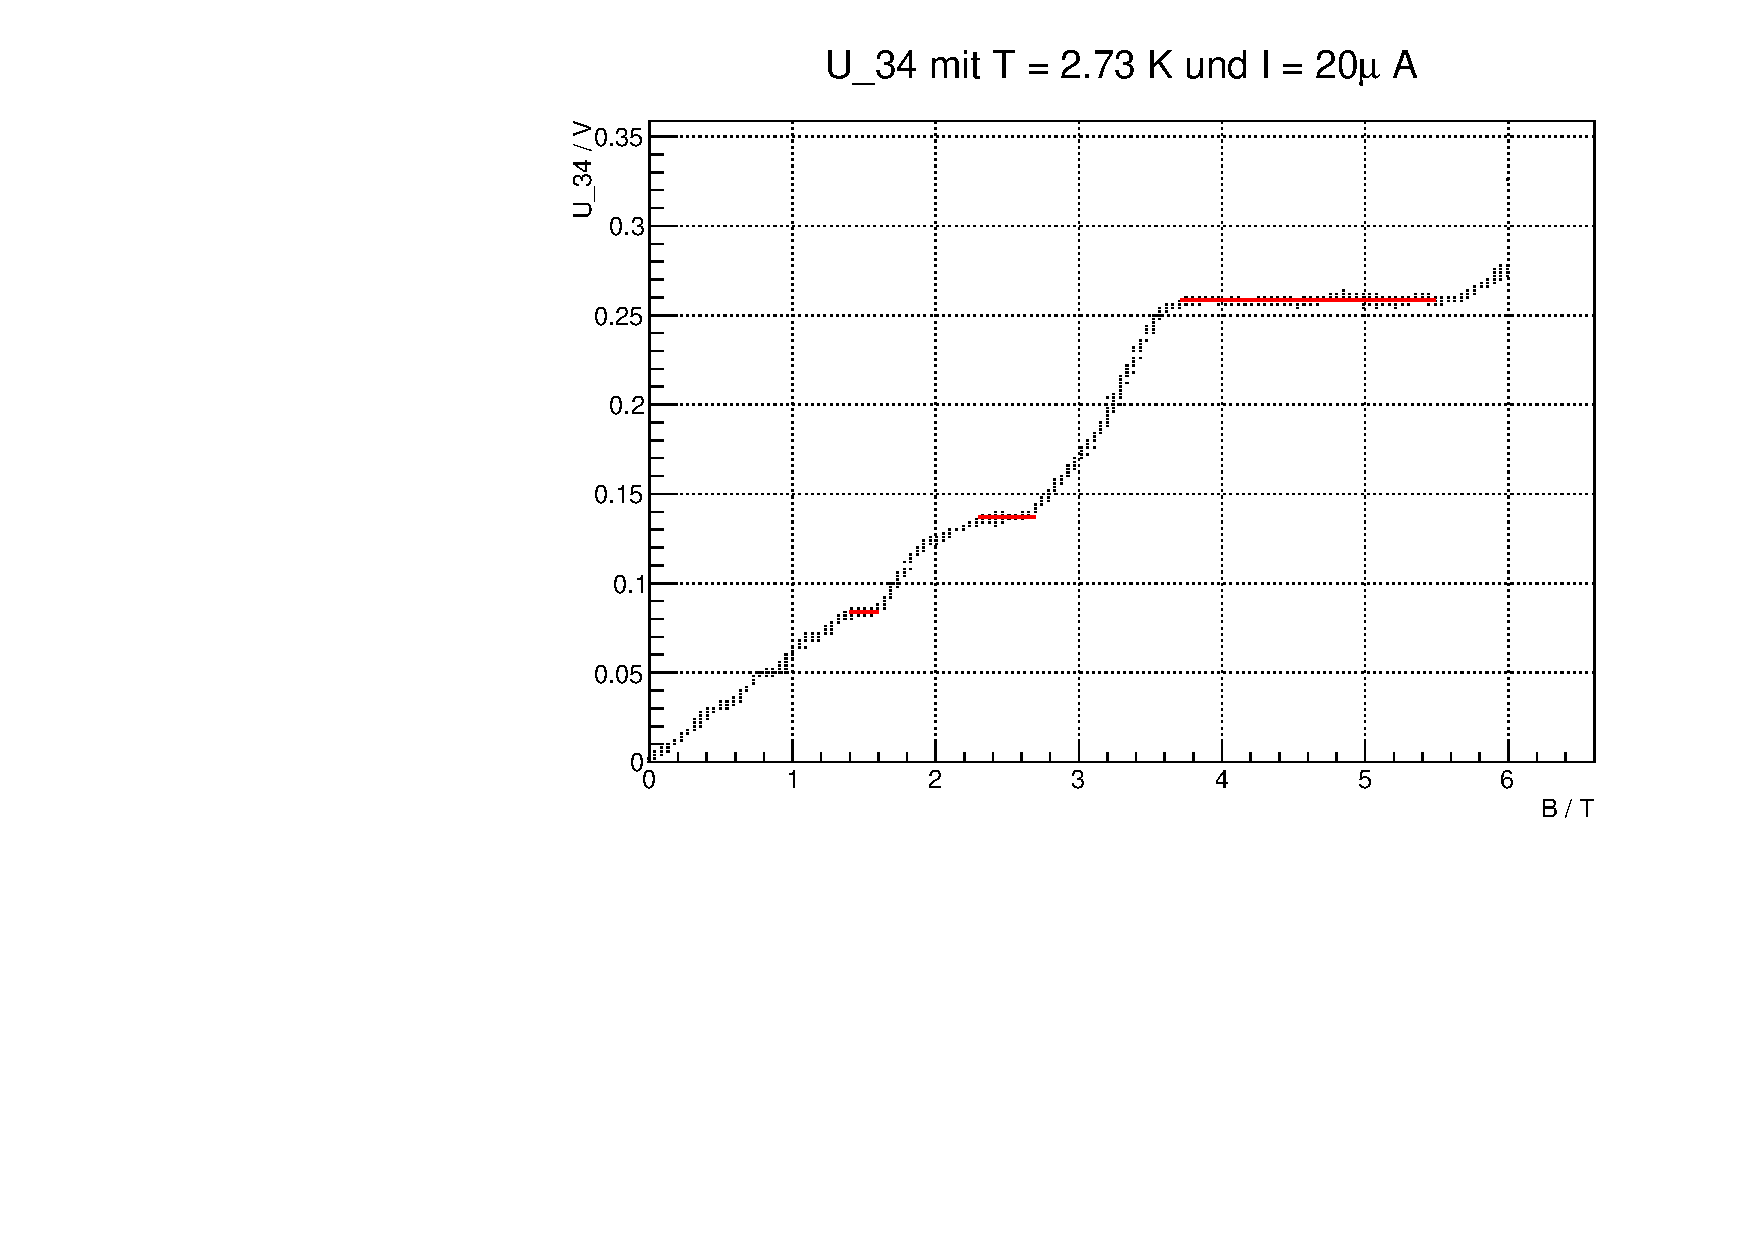
\includegraphics[scale = 0.5]{../plots/U_34_20muA_2730mK.pdf}
\caption{Hallspannung $\text{V}_H$ für I=20 $\mu$A und T=2.73 K}
\end{figure}


%T_high I_low U_hall
%U1 = 0.131545 +- 0.000282565
%U2 = 0.263575 +- 0.000178472
\begin{figure}
\label{}
\centering
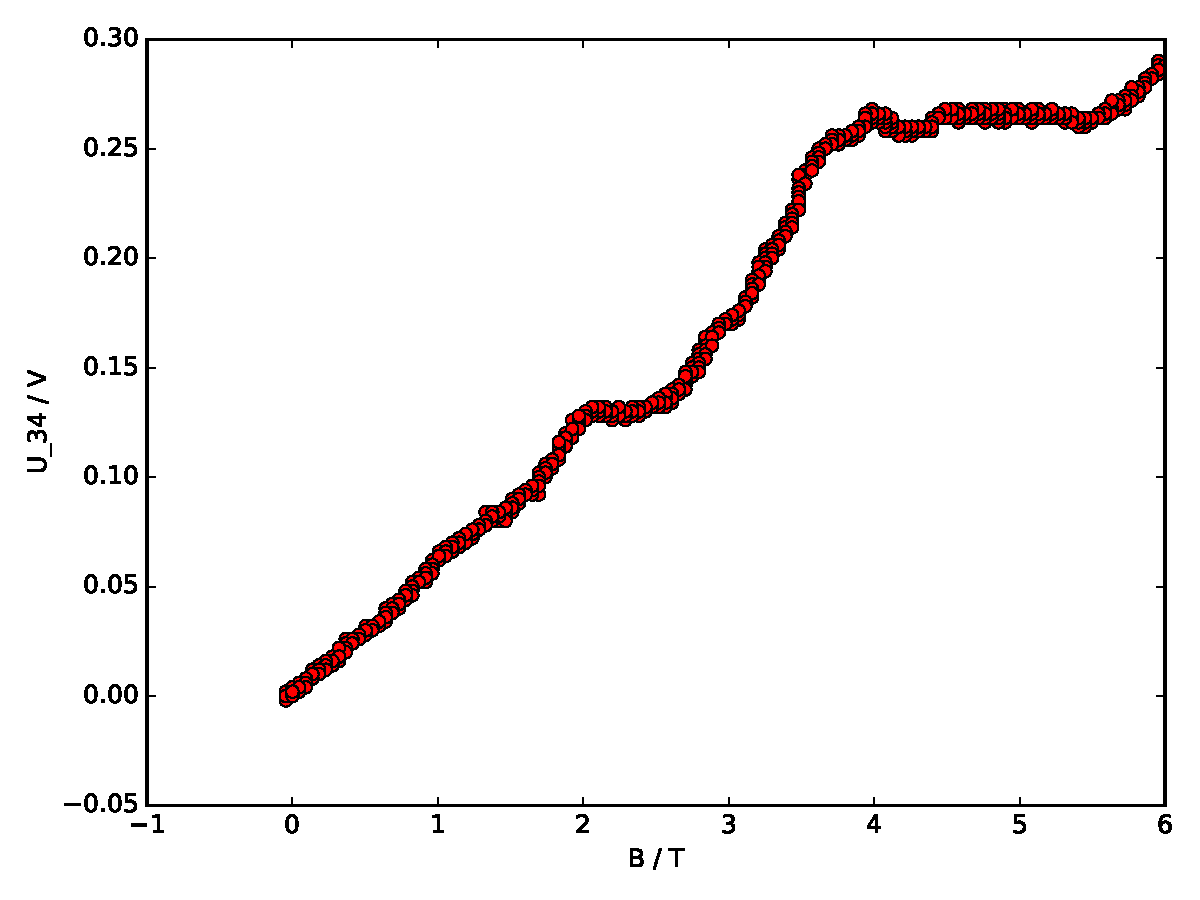
\includegraphics[scale = 0.5]{../plots/U_34_20muA_4100mK.pdf}
\caption{Hallspannung $\text{V}_H$ für I=20 $\mu$A und T=4.1 K}
\end{figure}


%T_low I_high U_hall
%U1 = 0.645867 +- 0.00088919
%U2 = 1.30603 +- 0.00025627
\begin{figure}
\label{}
\centering
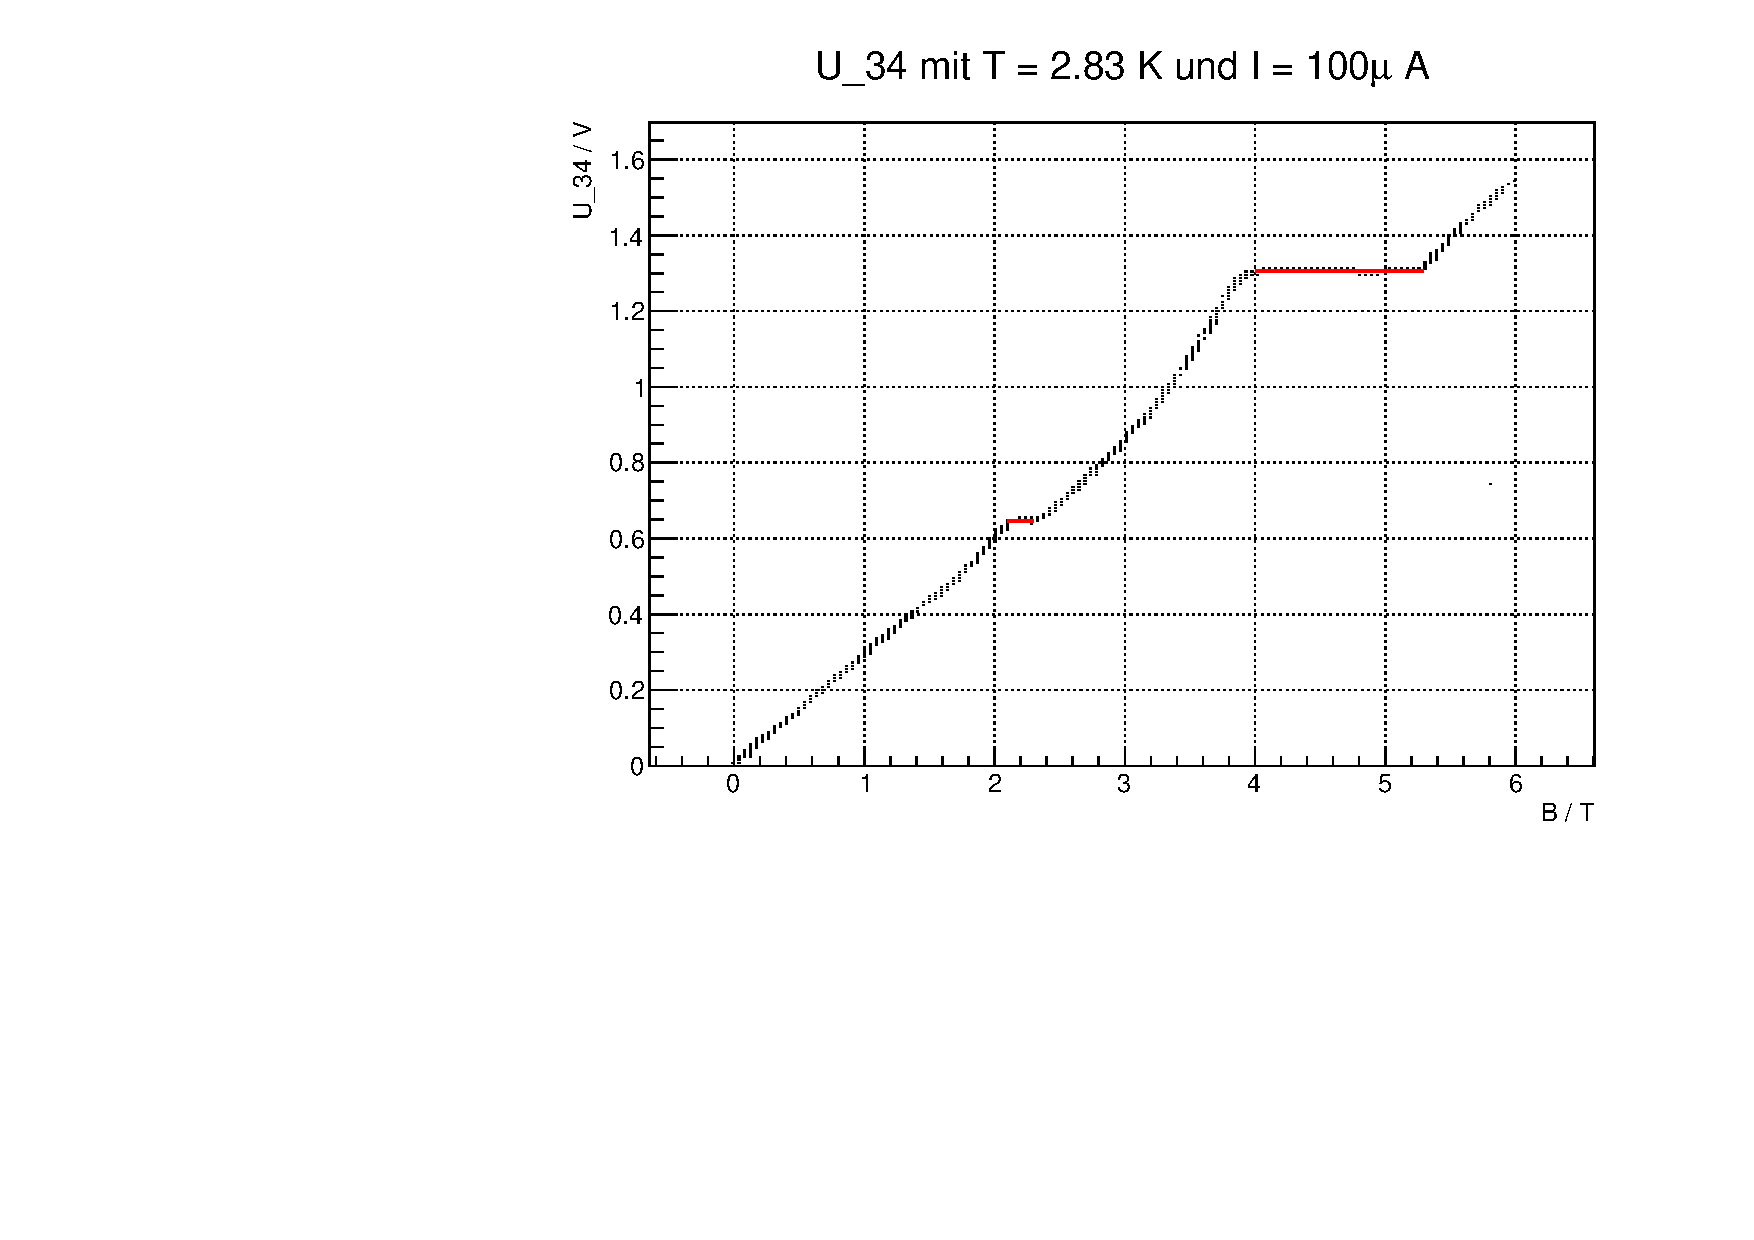
\includegraphics[scale = 0.5]{../plots/U_34_100muA_2830mK.pdf}
\caption{Hallspannung $\text{V}_H$ für I = 100 $\mu$A und T=2.83 K}
\end{figure}


%T_high I_high U_hall
%U1 = 0.656545 +- 0.00117472
%U2 = 1.30261 +- 0.000290939
\begin{figure}
\label{}
\centering
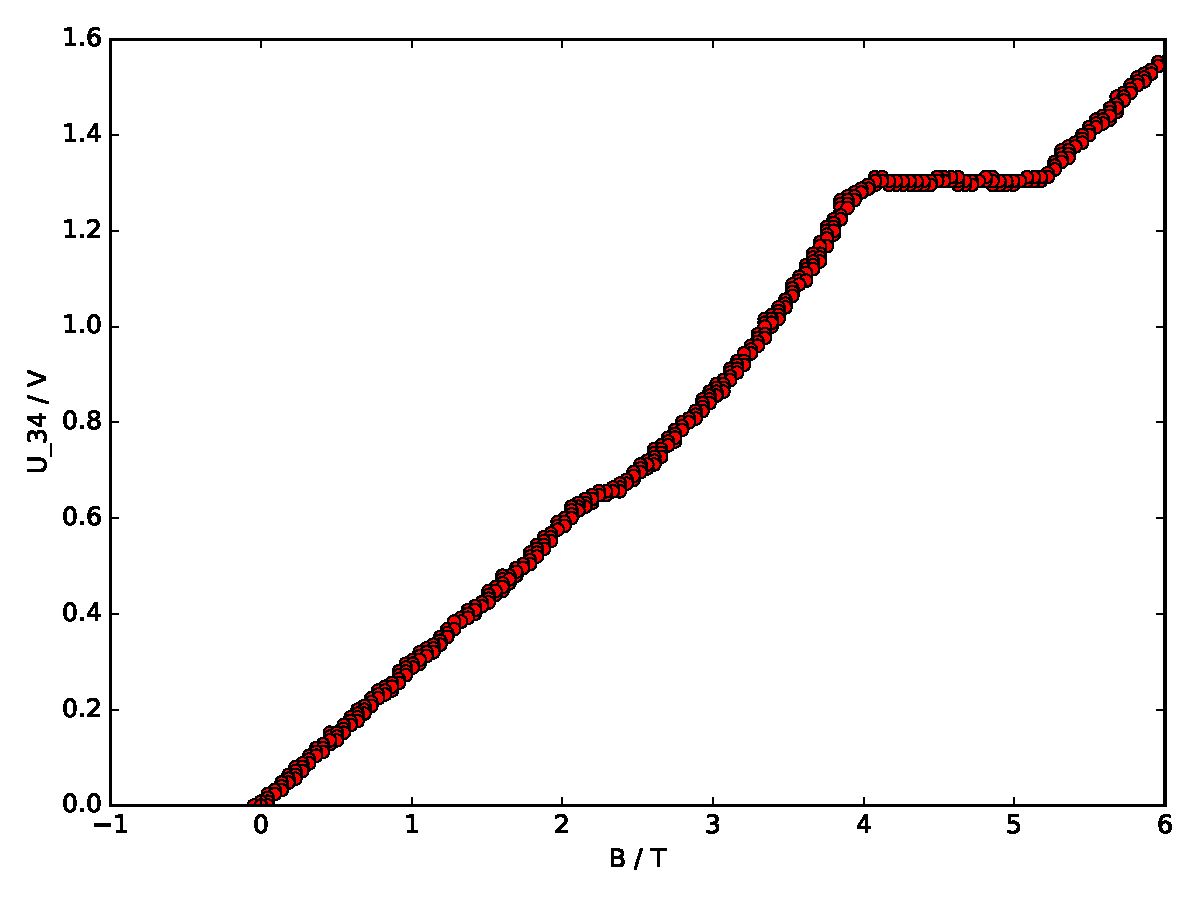
\includegraphics[scale = 0.5]{../plots/U_34_100muA_4400mK.pdf}
\caption{Hallspannung $\text{V}_H$ für I=100 $\mu$A und T=4.4 K}
\end{figure}




\FloatBarrier

\subsubsection{Identifikation der Plateuas}
Nach Vorbereitungsmappe gilt die Gleichung
$$\frac{U_H}{I} = \frac{h}{i \cdot e^{2}} $$
mit der Hallspannung $U_H$, dem angelegten Strom I und dem Füllfaktor i. In obiger Tabelle, Abb.5, ist dieser Füllfaktor für jedes Plateau mit angegeben. Dabei wurde die Bedingung ausgenutzt, dass i eine ganze Zahl sein muss; bei der Berechnung lag diese Zahl aber nie weiter als eine Standardabweichung von dem ungerundeten Wert entfernt.

\subsubsection{Ladungsträgerkonzentration}
Die Flächenladungsträgerdichte $n_s$ eines 2DEG wird berechnet aus
$$U_H = \frac{B}{n_s \cdot e} \cdot I $$
Sie ist quantisiert und abhängig von dem jeweiligen Hall-Plateau.

\subsection{Feinstrukturkonstante}
Die Feinstrukturkonstante wird wie in der Vorbereitung erwähnt berechnet durch folgende Gleichung:
$$\frac{U_H}{I} = \alpha ^{-1} \cdot \mu _0 c / (2 \cdot i) $$
Zur Berechnung der Messunsicherheit wird für die Hallspannung $U_H$ obige Wert aus den Fits verwendet. Die Stromstärke ist mit dem verwendeten Gerät in diesem Bereich sehr genau einstellbar, weswegen die Messunsicherheit darauf vernachlässigt wird. \\
Für die magnetische Feldkonstante und die Lichtgeschwindigkeit werden die Werte aus der Vorbereitungsmappe verwendet:
$$\mu _0 = 4 \pi \cdot 10^{7} \ NA^{-2} $$
$$c = 299792 \ \frac{m}{s} $$
Damit wird für jedes Hall-Plateau ein Wert für $\alpha$ berechnet und in einen Graphen eingetragen. Das ist in Abb.10 zu sehen. Es wurde noch eine Ausgleichsgerade gefittet und der theoretische Wert von $\alpha _{theo} = \frac{1}{137} \approx 7.299 \cdot 10^{-3}$ eingezeichnet. Die Feinstrukturkonstante haben wir somit bestimmt zu:
$$\alpha = (7.228 \pm 0.001) \cdot 10^{-3}$$

\begin{figure}
\centering
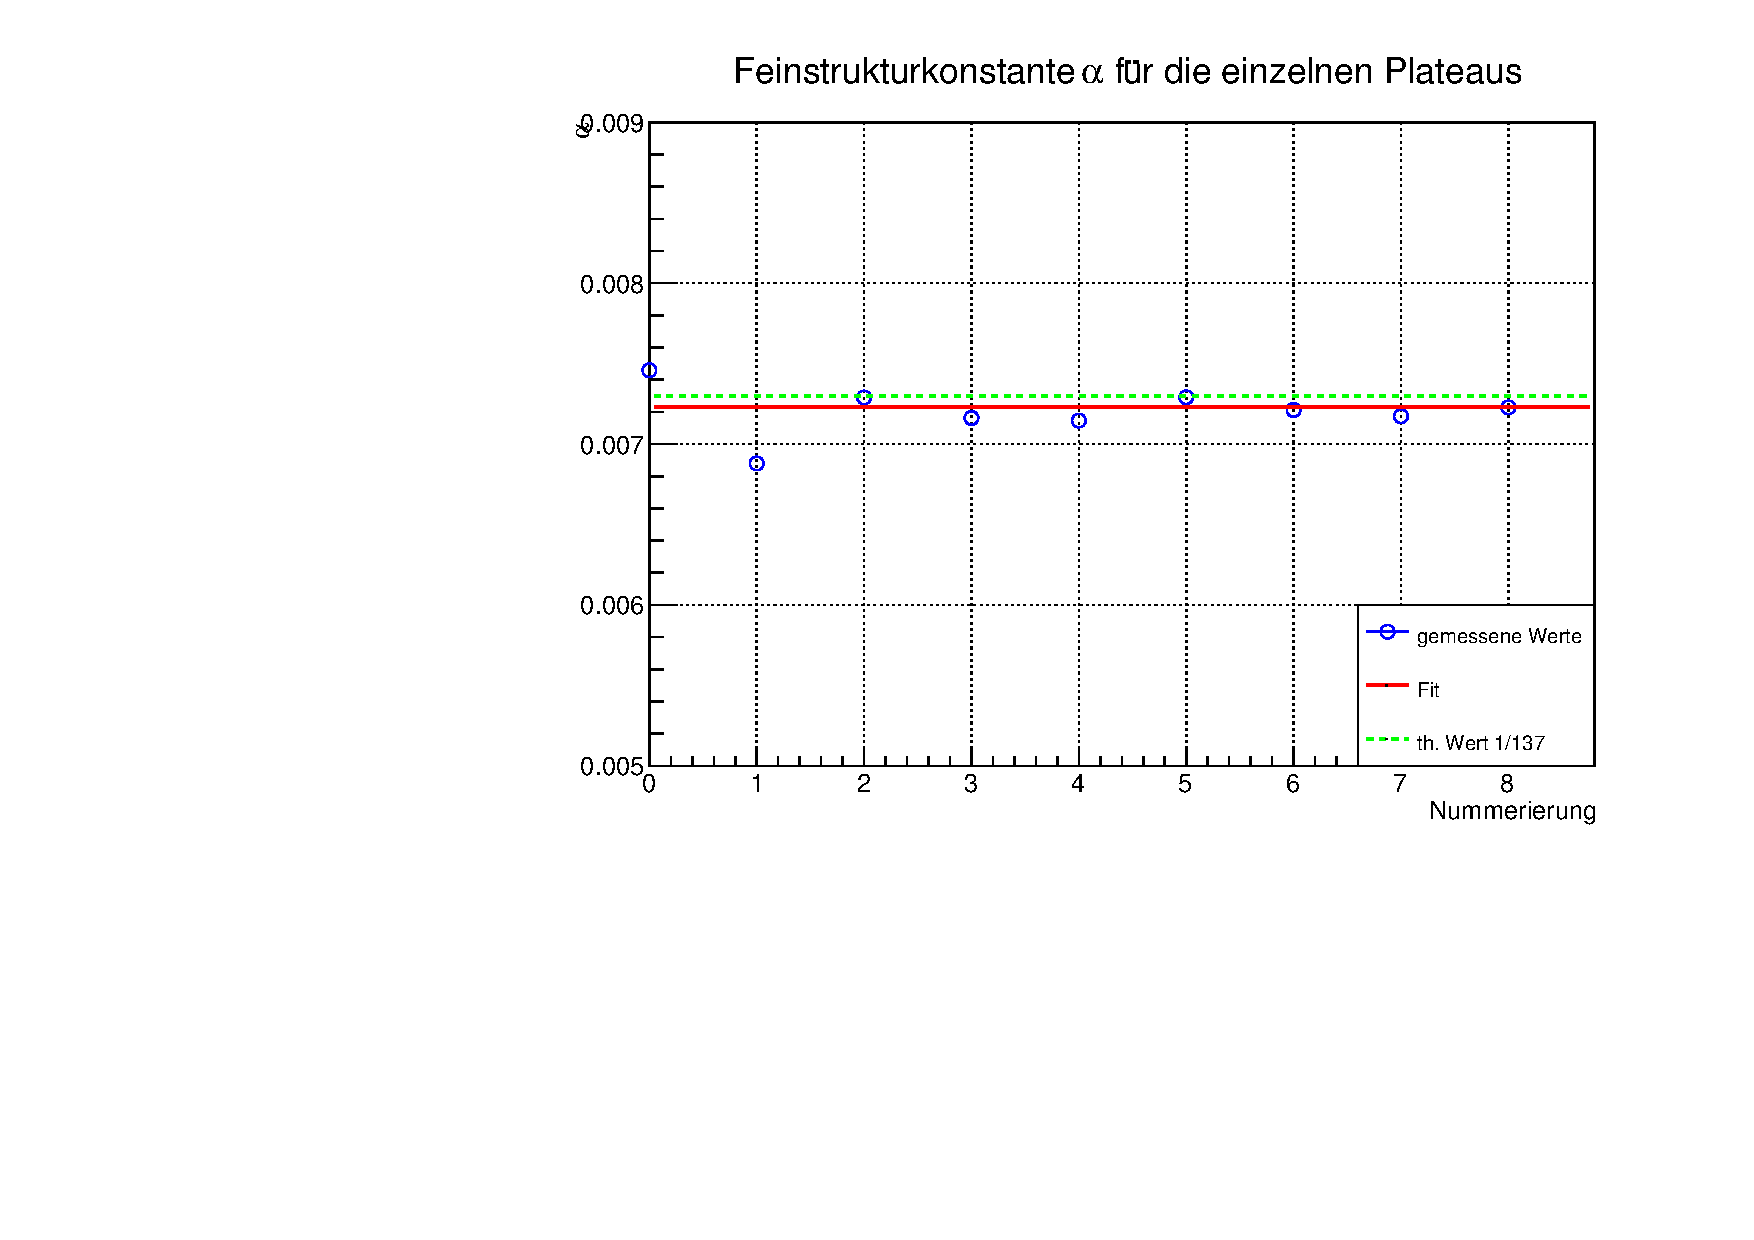
\includegraphics[scale=0.5]{../plots/alpha.pdf}
\caption{Feinstrukturkonstante $\alpha$ für jedes Plateau und horizontaler Fit. Gestrichelt ist der theoretische Wert von ungefähr $\frac{1}{137}$ eingezeichnet. Die Nummerierung ist analog zu Abb.5. Oberster Eintrag in der Tabelle entspricht dem Wert mit der kleinsten Nummerierung.}
\end{figure}

\subsection{Literaturvergleich}
Der theoretische Wert der Feinstrukturkonstanten liegt mehr als eine Standardabweichung von unserem Ergebnis entfernt. Die relative Abweichung ist allerdings sehr gering. Da die Feinstrukturkonstante keine wirkliche Konstante ist und ihren Wert von dem betrachteten Energiebereich ändert und da der Wert von $\frac{1}{137}$ nur eine ungefähre Angabe ist, ist das Ergebnis zufriedenstellend.